
\chapter{Generation} \label{generation}

\begin{figure}
	\centering
		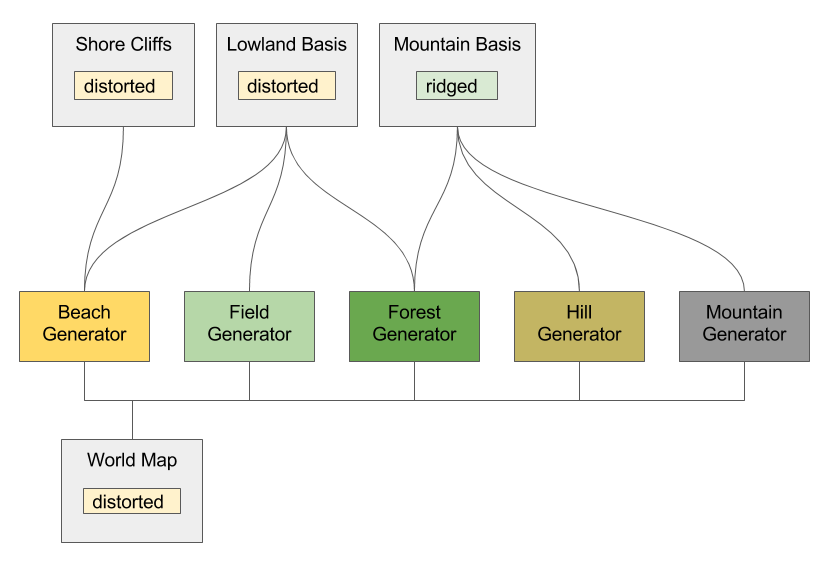
\includegraphics[width=1.0\textwidth]{figures/generation_flowchart.png}
	\caption{Terrain generation system overview, showing the type of noise generators used.}
	\label{fig:gen_overview}
\end{figure}

Our terrain generation algorithm creates a world with large continents that contain beaches, forests, hills, and mountains.
The algorithm uses a low-frequency world map to determine continent outlines and region boundaries.
For finely sampled terrain values, the values of the world map are used to select and influence custom generators for each region type.
See Figures \ref{fig:gen_overview} and \ref{fig:worldmap}.
The world map is discussed in Section \ref{sec:worldmap} and the different region generators are discussed in \ref{sec:region}

\begin{figure}
	\centering
		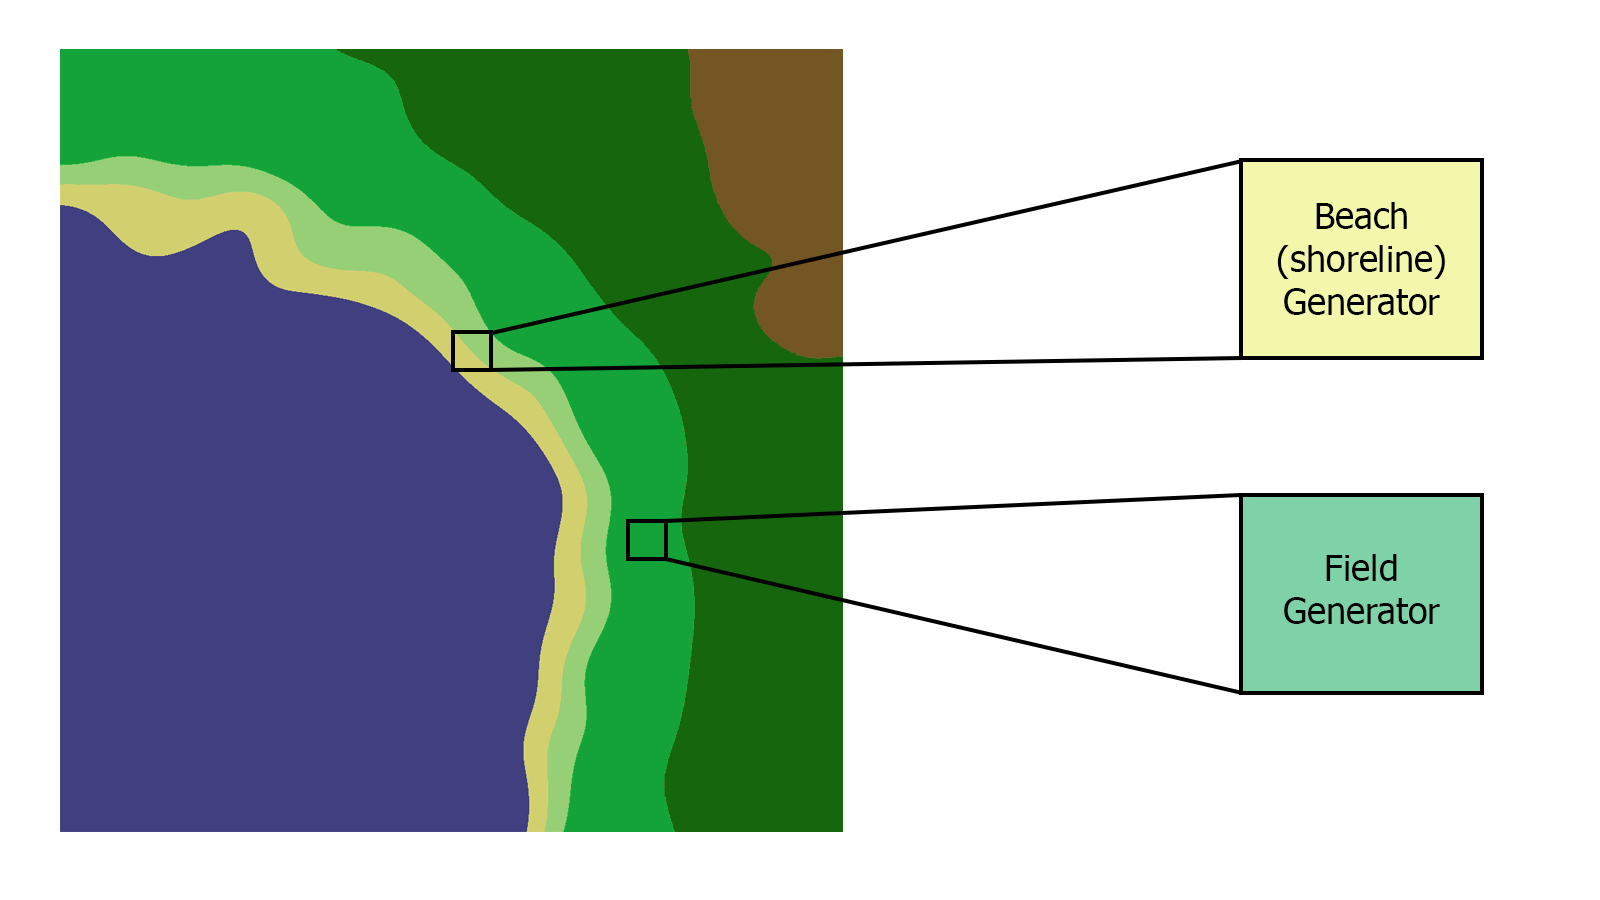
\includegraphics[width=1.0\textwidth]{figures/worldmap.png}
	\caption{Example world map section and generator selection.}
	\label{fig:worldmap}
\end{figure}

\section{World Map} \label{sec:worldmap}

The terrain is generated by first establishing a low-frequency world map, then selecting from a series of different landscape generators based on general elevation.
The world map uses a single distorted fractal noise layer with a box ramp to force oceans at all borders.

A low number of octaves is used (four, in our implementation) to guarantee a lack of high-frequency details.
This makes it useful for generating features without having areas that swap between multiple region types unrealistically.
Figure \ref{fig:worldmap} shows an example of the smooth isolines generated by the world map.

\section{Regions} \label{sec:region}

For rendering, the terrain values need to be generated at 1 foot postings.
We also need color values to shade the ground, and a forestation value to determine how to place trees.

Values from the world map are used to pick a particular set of terrain generation rules, referred to as a region.
The return value from the world map generator has a theoretical range from -1 to 1, but most values tend to be between -0.7 and 0.7.
This range is divided into regions with low values mapping to low elevation regions and high values mapping to high elevation regions.
See \ref{tab:regions} for the exact world map values used to determine regions.

\begin{table}
	\centering
	\begin{tabular}{ || c | c | c || }
		\hline
		Region & Minimum & Maximum \\ [0.5ex]
		\hline\hline
		Ocean & -1 & 0 \\
		\hline
		Shore & 0 & 0.05 \\
		\hline
		Field & 0.05 & 0.15 \\
		\hline
		Forest & 0.15 & 0.30 \\
		\hline
		Hills & 0.30 & 0.45 \\
		\hline
		Mountain & 0.45 & 1.0 \\ [1ex]
		\hline
	\end{tabular}
	\caption{Region boundaries from the world map values.}
	\label{tab:regions}
\end{table}

The world map can usually be used to generate color values, i.e. the color from the image in \ref{fig:worldmap} is used by each region generator.
However, the Mountains generator in Section \ref{sec:mountains} does some additional coloring.

For each region, a ``region delta'' is calculated to indicate how far into a region the engine is currently generating data for.
A region delta of \(0.0\) indicates the boundary with the next lower elevation region, \(1.0\) indicates the higher boundary, and \(0.5\) indicates the middle of the region.

The region types used by the engine are: Oceans, Beaches, Fields, Forests, Hills, and Mountains.

While each region generator is individually responsible for generating elevation values, some noise sources are shared between the different regions so that smooth transitions can be generated.
As an example, the Oceans, Fields, and Forests generators all share a distorted fractal noise source.

\subsection{Oceans and Fields}

The oceans, fields, and forests generators all simply add some high-frequency noise to the world map value with some scaling.
This generates small sandy hills below water for Oceans, small grassy hills for Fields, and tree-covered hills for Forests.

\subsection{Beaches}

Beaches serve as a transition between oceans and fields.
Beaches may contain a cliff partway between the shoreline and the transition to the field region.

This cliff is generated by applying a vertical offset to any baseline value above a certain threshold.
The offset is applied gradually over a small area so that the cliffs are not completely abrupt, but have a horizontal dimension of a few feet.
As the baseline elevation approaches the transition to Fields, the offset is tapered off to give cliffs some additional prominence.
See Figure~\ref{fig:beach_cliffs}.

The cliff generation offset function is as follows, where v is the map value:

$$
shoreline(v) = \left\{\begin{array}{lr}
	0, & \text{for } 0 \leq x \leq \text{cliff\_start} \\
	\text{cliff\textunderscore size} * \text{cliff\_falloff} * \text{cliff\_gain}, & \text{for } \text{cliff\_start} < x \leq 1
\end{array}\right\}
$$

Where cliff\_gain and cliff\_falloff are both computed as follows, but clamped from 0 to 1:

$$
\text{cliff\_gain} = \frac{v - \text{cliff\_start}}{\text{cliff\_range}}
$$

$$
\text{cliff\_falloff} = \frac{x - (\text{cliff\_start} + \text{cliff\_range})}{\text{falloff\_range}}
$$

The exact size, shape, and shoreline distance of the cliffs are configured by the parameters cliff\_start, cliff\_range, cliff\_size, and falloff\_range.
Relic uses additional noise layers to add variance to these parameters, and adds applies a gain function to both cliff\_gain and cliff\_falloff to create a smoother final appearance.

\begin{figure}
	\centering
		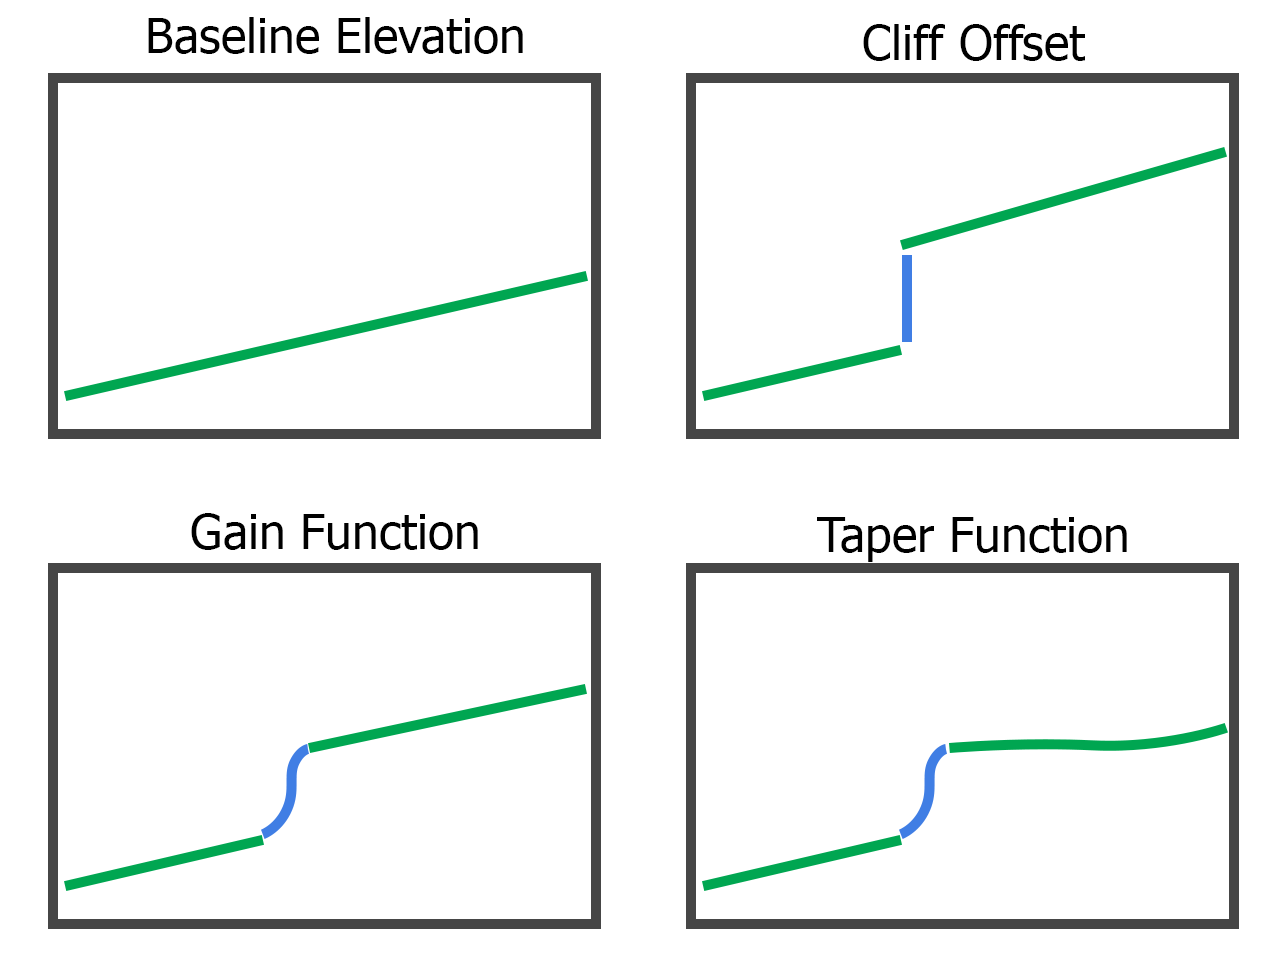
\includegraphics[width=0.8\textwidth]{figures/beachcliffs4x4}
	\caption{Beach cliff generation}
	\label{fig:beach_cliffs}
\end{figure}

\subsection{Forests, Hills, and Mountains} \label{sec:mountains}

The Forests, Hills, and Mountains regions both use a custom version of a ridged fractal generator.

For the first two octaves of noise, a standard gradient noise sample is used instead of the ridged version.
This helps reduce the sharpness of some peaks and hides some unnatural artifacts that sometimes occur.
Figure \ref{fig:original_ridged} shows the first few octaves of a ridged fractal generator without this modifications.
The ridge lines established by the second octave have a large effect on the resulting image even as more octaves are added.
The smoothness of these lines creates circular artifacts in the resulting terrain.
Figure \ref{fig:my_ridged} shows the first few octaves of a ridged fractal generator with this modification.
The effect is similar to lowering the amplitude and increasing the frequency of a normal ridged fractal generator but with large-scale variation preserved.

\begin{figure}
	\centering
		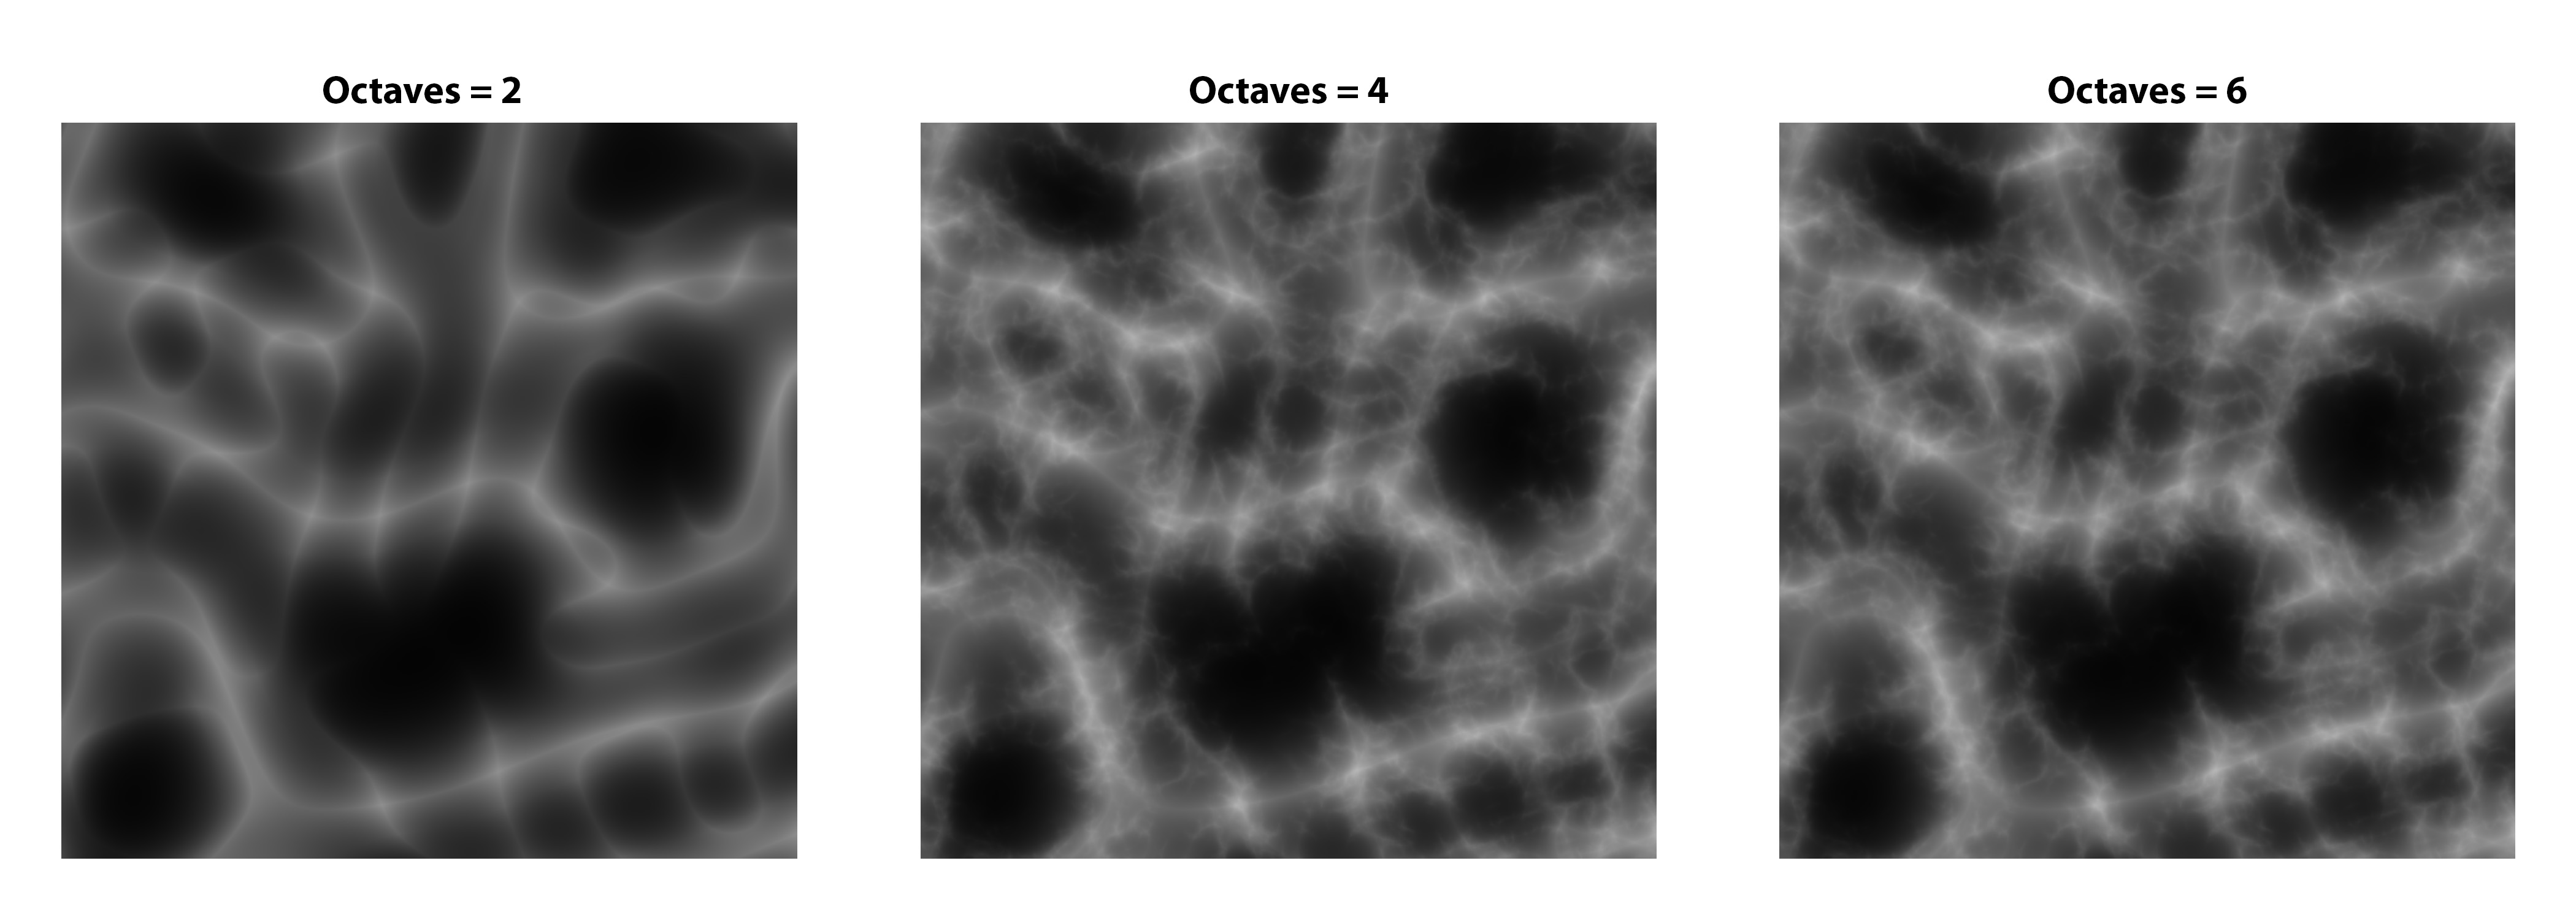
\includegraphics[width=1.0\textwidth]{figures/original_ridged}
	\caption{Two, Four, and Six octaves of a standard ridged fractal generator without our modification of using a standard fractal noise source for the first two octaves.}
	\label{fig:original_ridged}
\end{figure}

\begin{figure}
	\centering
		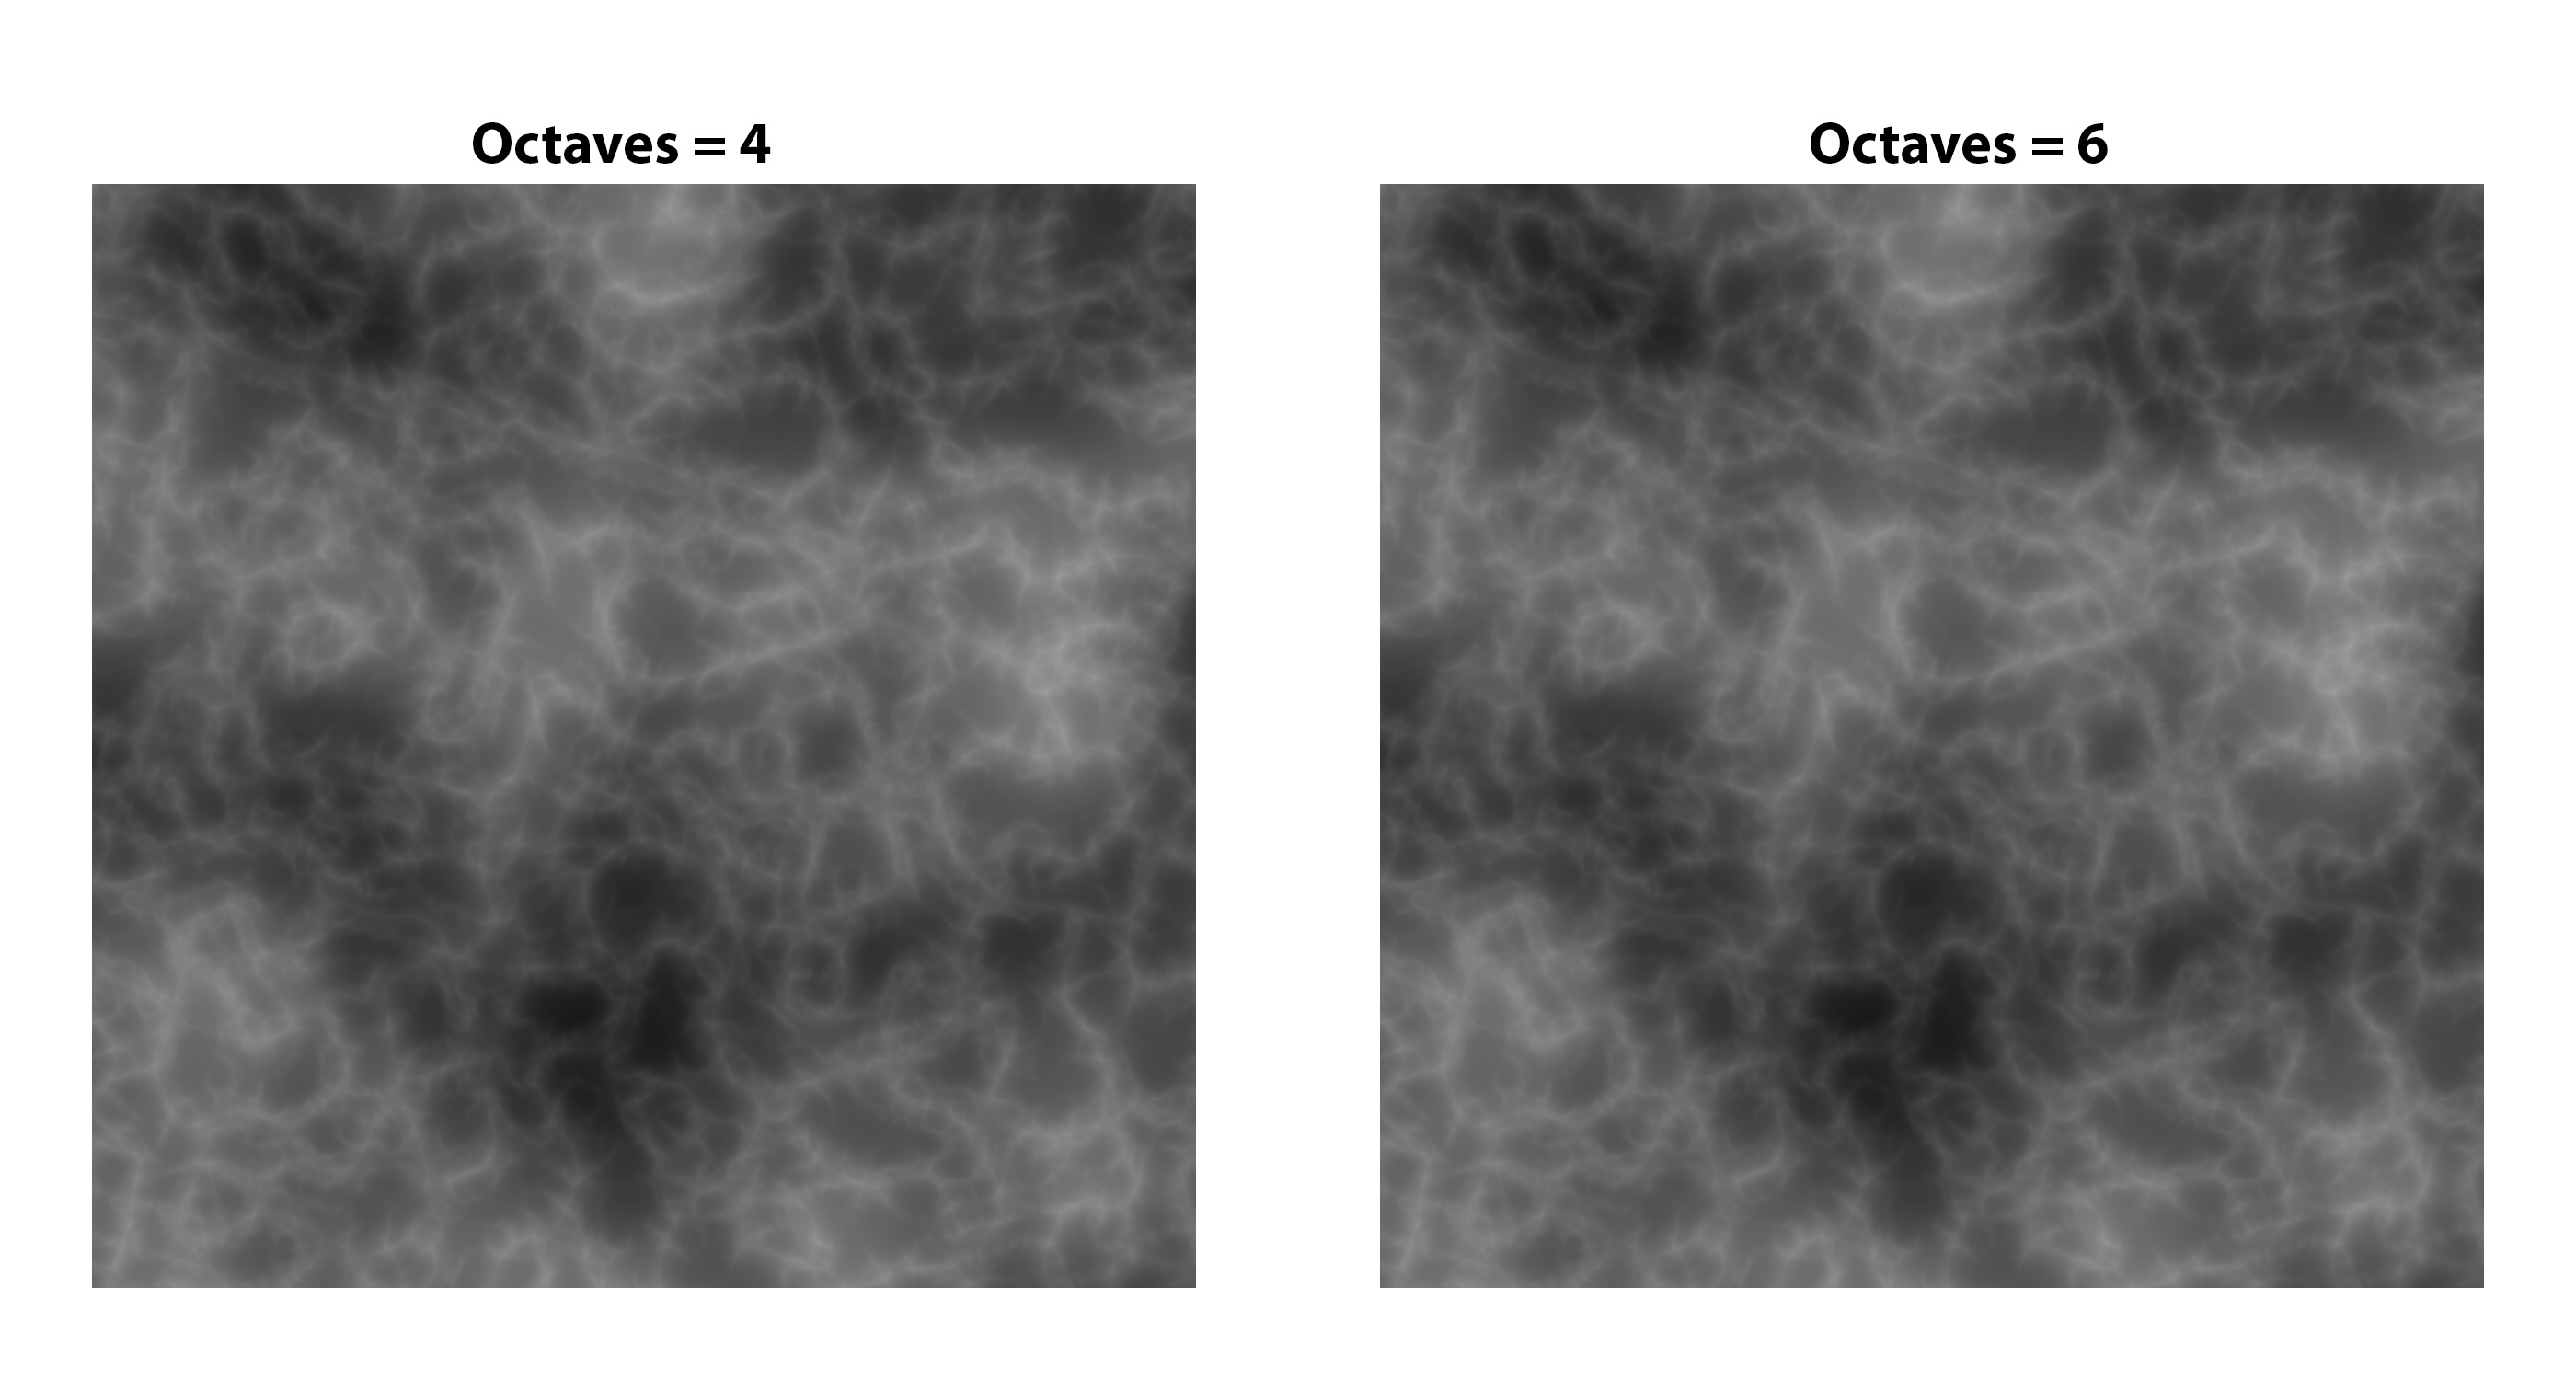
\includegraphics[width=1.0\textwidth]{figures/my_ridged}
	\caption{Four and Six octaves of the ridged fractal generator used by Relic, where a standard fractal noise source is used for the first two octaves.}
	\label{fig:my_ridged}
\end{figure}

In addition, a hilliness parameter is added to help smoothly transition between mountains and hills.
When hilliness is 0, the standard absolute value is used.
At hilliness of 1, the input value is squared instead to produce a parabolic shape.
Hilliness values between 0 and 1 interpolate between these two shapes.

At the low edge of Hill regions, a hilliness value of 1 is used along with low overall amplitude.
These same parameters are used at the high edge of the Forest region, and create smooth rolling hills of medium height.
In the Mountain region, hilliness falls to 0 and amplitude increases to create sharp ridge lines and towering peaks.

Mountain regions are colored by adding snow coverage over the region color specified by the world map.
Snow is added whenever the angle between the normal of the surface and the up vector is smaller than some value.
For high elevations, a large angle is used, and at low elevations a small angle is used.

\section{System Overview}

The use of a world map generator defines at a large scale what type of geometry to generator, including continent outlines and region boundaries.
Values generated by the world map are used to pick a particular region generator and transition smoothly between each region.
The regions, in order of elevation, are Oceans, Beaches, Fields, Forests, Hills, and Mountains.
Oceans and Fields have simple geometry - just some low amplitude noise to create small hills and variations.
Beaches serve as a ramp between Ocean and Field regions, with a cliff generated partway up the shore.
Forests, Hills, and Mountains use a custom ridged fractal generator to create ridged mountaintops and rolling hills.
